% spectral theorem
\documentclass[tikz,border=1pt]{standalone}
\usetikzlibrary{shapes.geometric}

\tikzstyle{start} = [rectangle,rounded corners,minimum width=3cm,minimum height=1cm,draw=black,text centered,fill=red!20]
\tikzstyle{condi} = [ellipse,text width=3cm,draw=black,text centered,fill=blue!20]
\tikzstyle{state} = [rectangle,text width=3cm,draw=black,text centered,fill=green!20]
\begin{document}
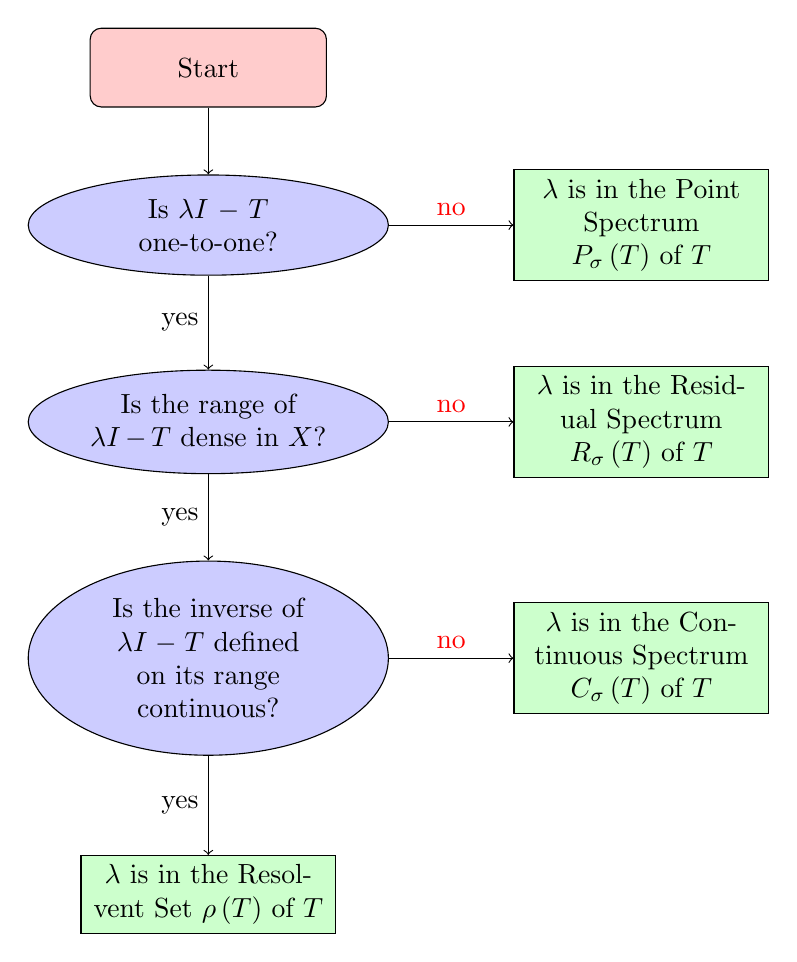
\begin{tikzpicture}[node distance=2cm]
    % Start
    \node[start] (start) {Start};
    
    % Conditions
    \node[condi,below of=start] (Q1) {Is $\lambda I - T$ one-to-one?};
    \node[condi,below of=Q1,yshift=-0.5cm] (Q2) {Is the range of $\lambda I - T$ dense in $X$?};
    \node[condi,below of=Q2,yshift=-1cm] (Q3) {Is the inverse of $\lambda I - T$ defined on its range continuous?};
    
    % Statements
    \node[state,right of=Q1,xshift=3.5cm] (S1) {$\lambda$ is in the Point Spectrum $P_{\sigma}\left(T\right)$ of $T$};
    \node[state,right of=Q2,xshift=3.5cm] (S2) {$\lambda$ is in the Residual Spectrum $R_{\sigma}\left(T\right)$ of $T$};
    \node[state,right of=Q3,xshift=3.5cm] (S3) {$\lambda$ is in the Continuous Spectrum $C_{\sigma}\left(T\right)$ of $T$};
    \node[state,below of=Q3,yshift=-1cm] (S4) {$\lambda$ is in the Resolvent Set $\rho\left(T\right)$ of $T$};

    % arrow
    \draw[->] (start) -- (Q1);
    \draw[->] (Q1) -- node[anchor=east] {yes} (Q2);
    \draw[->] (Q2) -- node[anchor=east] {yes} (Q3);
    \draw[->] (Q1) -- node[anchor=south] {\textcolor{red}{no}} (S1);
    \draw[->] (Q2) -- node[anchor=south] {\textcolor{red}{no}} (S2);
    \draw[->] (Q3) -- node[anchor=south] {\textcolor{red}{no}} (S3);
    \draw[->] (Q3) -- node[anchor=east] {yes} (S4);
\end{tikzpicture}
\end{document}